\section{Exact asymptotic description}
\label{2406:sec:main:warm_start}
We now characterize the exact asymptotic description of the dynamics of two-layer networks trained with SGD. In Figure~\ref{2406:fig:warm_start_pd} we sketch a representative phase diagram as a function of the relevant parameter of the algorithm, i.e. the learning rate and the batch size. The plot identifies different regions of parameters defining the network's learning efficiency.
% Moreover, we offer numerical evidences showing that, although not described provably, the closed-form equations capture the dynamics also in the cold start regime. 

\paragraph{Sufficient statistics ---}
Our study, like many other efforts \citep{arous2022high,saad1995line}, is based on the concentration of the neurons' overlaps with the target subspace and their norms. This approach only requires the knowledge for every optimization step $t \in [T]$ of the above defined overlaps, often referred to as \textit{sufficient statistics}. Let the pre-activations be defined as:
\begin{align}
    \vec \lambda_t = W_t \vec z \qquad  \text{and} \qquad \vec \lambda^\star = W^\star \vec z
\end{align}
Thanks to the Gaussian nature of the data, the pre-activations at any time step $t$ are jointly Gaussian vectors $(\vec{\lambda}_t, {\vec{\lambda}^{\star}})\sim\mathcal{N}(\vec{0}_{p+k}, \Omega_t)$ with covariance
$\Omega_t \in\mathbb{R}^{(p+k)\times (p+k)}
$: 
\begin{equation}
\label{2406:eq:main:covariance_def}
\Omega_t \coloneqq
\begin{pmatrix}
Q_t & M_t\\
{M_{t}^\top} & P
\end{pmatrix}=
\begin{pmatrix}
W_t{W_t}^{\top} & W_t{W^{\star}}^{\top}\\
W^{\star}W_{t}^\top & W^{\star} W^{\star \top}
\end{pmatrix}
\end{equation}
We refer to $M_t,Q_t$ as the \textit{order parameters}.
\begin{figure*}
    \centering
    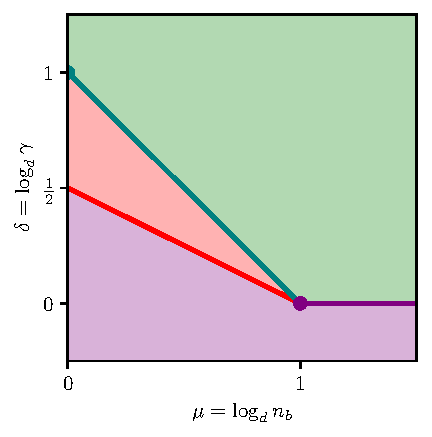
\includegraphics[width=0.445\textwidth]{figs/exact_asymptotic_diagram_no_legend}
    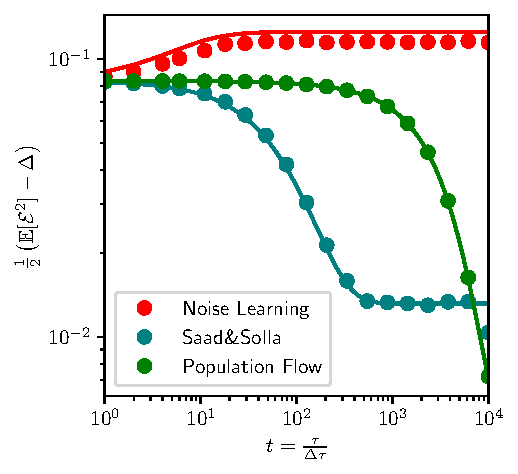
\includegraphics[width=0.49\textwidth]{figs/dynamicsH3_multindex}
    \caption{\textbf{Exact asymptotic description:}
        Exact asymptotic characterization of the dynamics of two-layer networks trained with SGD as a function of the batch size ($n_b$) and the learning rate ($\gamma$). \textbf{Left:} Illustration of the different dynamical regimes in a compact phase diagram. \textbf{\color{allowedcolor} Population flow region:} The dynamics is equivalent to population gradient flow. \textbf{\color{notallowedcolor} Noise learning region:} The high-dimensional noise terms dominate the dynamics. 
        \textbf{\color{teal} Saad~\&~Solla line:}
        The learning dynamics attains a plateau characterized by the noise variance \cite{saad1995line}. \textbf{\color{nodynamicscolor} Dynamics not defined:} The deterministic low-dimensional description of the Equation~\eqref{2406:eq:spherical_closed_form_ode} is not valid.
        \textbf{Right:} The figure shows a comparison of numerical simulations (dots) and theoretical prediction (continuous lines) for three instances $(\delta,\mu)$ associated with different learning regimes (identified by the corresponding colors). For both theory and simulations, the test error is plotted as a function of SGD iterations. We consider a matching architecture problem, i.e. \(\ h^\star = \sigma = \erf\) activation, and hidden units \(p=2,k=2\).
    }
    \label{2406:fig:warm_start_pd}
\end{figure*}
\subsection{Closed form equations}
We are now in the position to state our proposition that
provides a set of deterministic ODEs to describe one-pass SGD in high-dimensions.
This portrayal depends ultimately only on the values of the learning rate and the batch size, as quantified by the exponents \((\delta, \mu) \). 
\begin{proposition}
\label{2406:prop:main:exact_asympt}
% The projected SGD dynamics over the weights in Equation~\eqref{2406:eq:main:gd_update_weights} describes a dynamical process for the order parameters that converges to a coupled set of low-dimensional deterministic equations. 
Consider \(\bar\Omega(t)\) the solution of the system of ordinary differential equations
\begin{equation}
\label{2406:eq:spherical_closed_form_ode}
\begin{split}
    \dod{M_{jr}}{\tau} =& \Psi_{jr}{(\Omega)} - \frac{M_{jr}}{2}\Phi_{jj}{(\Omega)} \\
    \dod{Q_{jl}}{\tau} =& \Phi_{jl}{(\Omega)} - \frac{Q_{jl}}{2}\left(\Phi_{jj}{(\Omega)} + \Phi_{ll}{(\Omega)}\right)
\end{split}
\end{equation}
where we introduced:
\begin{equation}
\label{2406:eq:informal_ODE}
\begin{split}
    \Psi_{jr}(\Omega) =&  \mathbf{1}_{\{\delta\ge0 \bigcap 2\delta+\mu\ge1\}}\frac{\gamma_0}{p}a_j \psi_{jr}  \\
    \Phi_{jl}(\Omega) =&  \mathbf{1}_{\{\delta\ge0 \bigcap 2\delta+\mu\ge1\}}\frac{\gamma_0}{p}\left(a_j^{t}\phi^{\rm{GF}}_{jl}+a_l^{t}\phi^{\rm{GF}}_{lj}\right) \\
        &+\mathbf{1}_{\{\delta+\mu\ge1 \bigcap 2\delta+\mu\le1\}}\frac{\gamma_0^2}{p^2n_0}a_j^{t} a_l^{t} \phi^{\rm{HD}}_{jl} 
        % \\
        % &+\mathbf{1}_{\{\delta=0,\mu\neq0\}}\frac{\gamma_0^2}{p^2} a_j^{t} a_l^{t}\phi^{\rm{BC}}_{jl}
\end{split}\end{equation}
and auxiliary integrals bearing expectations over $\mathcal{N}(\vec 0, \Omega)$:
\begin{align*}
    \psi_{jr} =&\mathbb{E}\left[ \sigma'(\lambda_j)\lambda^{\star}_{r} \mathcal{E} \right] \\
    \phi^{\rm{GF}}_{jl}=&\mathbb{E}\left[ \sigma'(\lambda_j)\lambda_{l} \mathcal{E} \right] \\
    \phi^{\rm{HD}}_{jl}=&\mathbb{E}\left[ \sigma'(\lambda_j)\sigma'(\lambda_l)\mathcal{E}^2  \right]  \\
    \mathcal{E} =& g_\star(\vec \lambda^\star) - \frac{1}{p} \sum_{j=1}^p a_j \sigma(\vec \lambda)
    % \\
    % \phi^{\rm{BC}}_{jl}=&
    %     \mathbb{E}\left[\sigma'(\lambda_j)\mathcal E \left(\lambda^\star\right)^\top\right]P^{-1}\mathbb{E}\left[\sigma'(\lambda_l)\mathcal E \lambda^\star\right]+\\
    %     &\mathbb{E}\left[\sigma'(\lambda_j)\mathcal E (\lambda^\bot)^\top\right]\left(Q^\bot\right)^{-1}\mathbb{E}\left[\sigma'(\lambda_l)\mathcal E \lambda^\bot\right] \\
    % 
\end{align*}
% and
% \[
% \vec \lambda^\bot = \vec \lambda - MP^{-1}\vec\lambda^\star
% \quad\text{and}\quad
% Q^\bot = Q - M P^{-1}M^\top.
% \]
Then, there exists a constant $C$ independent from the input data dimension, such that the discrete stochastic process for the covariance \(\{\Omega_t\}_{t\in\mathbb{N}}\) in Equation~\eqref{2406:eq:main:covariance_def} induced by projected SGD dynamics is approximated by the deterministic covariance matrix \(\bar\Omega(t)\) with precision:
\begin{equation}
\label{2406:eq:main:time_horizon}
    \mathbb{E} \norm{\Omega_t - \bar \Omega(t\Delta \tau)} \le e^{Ct}\sqrt{\Delta \tau} 
\end{equation}
with
    $\Delta \tau = d^{\max(-\delta,-2\delta+1-\mu)}$.
\end{proposition}
We refer to Appendix~\ref{2406:sec:app:derivation_of_lb_equations} for the informal derivation of the above result. 

In Figure~\ref{2406:fig:warm_start_pd}~(left) we summarize the results of Proposition~\ref{2406:prop:main:exact_asympt} in a compact phase diagram. 
The following dynamical regimes appear:
\begin{itemize}
    \item \textbf{Population Flow}: The dynamics of the sufficient statistics described by a deterministic set of ODEs~\eqref{2406:eq:spherical_closed_form_ode} is equivalent to population gradient flow. 
    \item \textbf{Noise learning}: The dynamic is dominated by high-dimensional noise, and consequently the algorithm does not learn the target;
        the behavior is reflected in the ODEs.
    \item \textbf{Saad~\&~Solla line}: The ODE description in Proposition~\ref{2406:prop:main:exact_asympt} is equivalent to the pivotal work on 2LNNs \cite{saad1995line}. In particular, the original work corresponds to the point \((\delta,\mu)=(1,0)\). The learning dynamics is blocked on a plateau characterized by the noise variance in the labels. 
    \item \textbf{Large batch interaction}: The dynamics is given by population gradient flow combined with the large-batch corrections terms, i.e. contributions coming from interaction between samples $\vec z^\nu, \vec z^{\nu'}$ in the same batch. This region corresponds in parameter space to \(\delta = 0, \mu > 1\).
    \item \textbf{Phase coexistent point}: The point \(\delta = 0, \mu = 1\) is the only point in parameter space where all term in the equations are not negligible.
    \item \textbf{Dynamics not defined}: For a broad range of values of \( (\delta, \mu) \) the SGD dynamics is not effectively described by a set of low-dimensional deterministic ODEs.
\end{itemize}
In the right panel of Figure~\ref{2406:fig:warm_start_pd} we present a numerical investigation of three particular instances of the regimes presented above. The plot shows a comparison of numerical simulations versus the low-dimensional exact asymptotic characterization given in Equations~\eqref{2406:eq:spherical_closed_form_ode}. The values of the learning rate and the batch size used for SGD training are varied to probe different regions of phase diagram~\ref{2406:fig:warm_start_pd}. 

\begin{remark}
When the target's leap index is $\ell>1$, the dynamic of SGD is dominated by a first extensive search phase to achieve weak recovery of the teacher direction (Theorem~\ref{2406:thm:main:sgd_weak_recovery}). 
% On the other hand, the ODE description for the dynamics in Proposition~\ref{2406:prop:main:exact_asympt} respects convergence bounds detailed in Equation~\eqref{2406:eq:main:time_horizon}. 
Therefore, in order to probe interesting dynamical regimes for general single index teachers, we assume non-vanishing initial correlations of the network's hidden layer weights with the teacher's ones when \(d\to+\infty\).

In Appendix~\ref{2406:sec:app:hyperparams} we study the tightness of the exponential bound Equation~\eqref{2406:eq:main:time_horizon}; we argue supported by numerical illustrations that (on the practical side) the low dimensional ODE description is valid well beyond the extents of Proposition~\ref{2406:prop:main:exact_asympt}, as already observed by other works \cite{goldt2019dynamics,veiga2022phase} in different context. 
\end{remark}



\paragraph{Non-asymptotic corrections ---}
Proposition~\ref{2406:prop:main:exact_asympt} unveils a surprising result for the exact asymptotic description of two-layer networks. Indeed, the ODEs written in Equation~\eqref{2406:eq:spherical_closed_form_ode} coincide with the analogous ones for the single sample per batch case ($n_b=1$), modulo trivial rescaling of the parameters \cite{veiga2022phase}.  However, a careful consideration of the self-interaction term in the gradient is needed for correctly describing the low-dimensional process of the order parameters:
\begin{align}
    \sum_{\nu' = 1, \nu'\neq\nu}^{n_b} \sigma'(\lambda_j^\nu)\sigma'(\lambda_l^{\nu'})\mathcal{E}^\nu\mathcal{E}^{\nu'} \langle \vec z^{\nu}, \vec z^{\nu'} \rangle 
\end{align}
The asymptotic form of this term can be exactly computed to be (using Proposition~\ref{2406:prop:main:exact_asympt} notations):
\begin{align}
\label{2406:eq:main:large_batch_term}
    \phi^{\rm{BC}}_{jl}=&\mathbb{E}\left[\sigma'(\lambda_j)\mathcal E \left(\lambda^\star\right)^\top\right]P^{-1}\mathbb{E}\left[\sigma'(\lambda_l)\mathcal E \lambda^\star\right]+\\
&\mathbb{E}\left[\sigma'(\lambda_j)\mathcal E (\lambda^\bot)^\top\right]\left(Q^\bot\right)^{-1}\mathbb{E}\left[\sigma'(\lambda_l)\mathcal E \lambda^\bot\right]
\end{align}
with $ \vec \lambda^\bot = \vec \lambda - MP^{-1}\vec\lambda^\star  \text{ and }  
Q^\bot = Q - M P^{-1}M^\top$.
Although the contribution of the above term is asymptotically vanishing in the ODE description~\eqref{2406:eq:spherical_closed_form_ode} when $d \to \infty$, any theoretical description at finite $d$ will effectively depend on $\phi^{\rm{BC}}_{jl}$. In Appendix~\ref{2406:sec:app:hyperparams} we provide additional numerical investigation on the importance of~\eqref{2406:eq:main:large_batch_term} and the role of large batch sizes for non-asymptotic corrections to the characterization in Proposition~\ref{2406:prop:main:exact_asympt}. Moreover, we note that taking into account the presence of large batch size is pivotal to illustrate the time~/~complexity tradeoffs for weak recovery of the target subspace, as thoroughly discussed in Section~\ref{2406:sec:main:cold_start}.
